\section{Experiments}
\label{sec:exp}

\paragraph{Protocol.}
Per benchmark we draw 30 repetitions of two splits (Table~\ref{tab:data}). In the \emph{random} split a fresh 25\% of the models are targets and the rest are sources. In the \emph{extrapolation} split the targets are the strongest 25\% of models by full accuracy, so that every source is weaker than every target; the partition is deterministic, and its repetitions vary the selector seed and an 80\% subsample of the sources. Budgets are $n\in\{10,20,50,100,200\}$, capped at $N/4$ (so $n{=}200$ exists for 8 of 13 benchmarks, and macro-averages are shown for $n\le 100$, where all 13 benchmarks are present). Exact duplicate model rows are collapsed before splitting (Appendix~\ref{app:data}); the target accuracy is always the mean over all $N$ items. Seeds derive from a hash of (benchmark, split, repetition, $n$, selector), so every method sees identical splits. Per (benchmark, split, $n$, repetition) we compute the four metrics over the target models, and report means with 95\% percentile-bootstrap intervals over repetitions (1000 resamples; the macro curves, tables and per-benchmark figures); paired differences are taken within repetition. These intervals describe the noise of the selector and of the source subsample with the target models fixed, not the choice of the 20--107 target models of a benchmark. For the headline paired differences to B1 (macro and per benchmark, $n\in\{20,50,100\}$, both splits) we therefore use a two-level bootstrap: repetitions are resampled and then the target models within each resampled repetition, with identical indices for every method so that differences stay paired (1000 resamples; the macro interval treats the 13 benchmarks as fixed, and they share models, so it does not cover variation over benchmarks). Compared with the repetition-only intervals, these are $2$--$48$\% wider (median $12$\%) at $n{=}50$, and no conclusion changed. We write TB for them where the distinction matters. Macro-averages weight the 13 benchmarks equally; the benchmarks share models, so they are not independent, and cross-benchmark statements are descriptive. A random subset of $n$ items has RMSE equal to its analytic standard error to within sampling noise, and $n=N$ reproduces the exact score (sanity checks in \texttt{results/sanity/}).

\paragraph{Freezing P3.}
P3 was designed on 3 benchmarks (IFEval, GSM8K, MMLU-Pro) with an inner split made only of source models and then frozen (Section~\ref{sec:methods}); the exploration that preceded it (a few 2--4 seed pilot runs on GPQA and MMLU-Pro with outer targets, used to build the candidate list) and a disclosure about reading the data repository's README are listed in Appendix~\ref{app:honest}. P3 is therefore not tuned on the evaluated targets, but its independence is partial.

\subsection{Random split: source-model information helps}
Table~\ref{tab:macro} and Appendix Figure~\ref{fig:paired} (right) answer Q1 for random splits. At $n=50$ the macro MAE of the random subset mean (B1) is $4.60\pm0.13$ points, and every source-informed method has a paired MAE difference to B1 whose TB interval excludes zero on the macro-average (intervals in Table~\ref{tab:ablation}): $-0.30$ (anchor points), $-1.44$ (Anchor+IRT), $-1.27$ (OMP+ridge), $-1.50$ (random+low-rank), $-1.56$ (P3 EB), $-1.20$ (P3 DR), $-0.88$ (B2) points. The gains are not uniform: at $n{=}50$, whether a benchmark's TB interval lies below zero is true for Anchor+IRT on 10 of 13 benchmarks and OMP+ridge on 8, and OMP+ridge is worse on three HELM benchmarks (Commonsense, GSM8K, MATH; Table~\ref{tab:perbench}). The gain shrinks with $n$ (Anchor+IRT: $-4.57$ points at $n{=}10$, $-0.74$ at $n{=}100$) because a random subset catches up. Rank correlations behave alike: at $n{=}10$ OMP+ridge has Spearman $0.87$ against $0.67$ for B1; at $n{=}100$ all methods are within $0.04$ of each other (Table~\ref{tab:macro}, Appendix Figure~\ref{fig:paired}). Anchor points, as we implemented them, are the weakest of the source-informed family and exceed B1 in MAE at $n\ge100$ (+0.21 at $n{=}100$).

\begin{table}[t]
\caption{Macro-average over the 13 benchmarks of MAE (accuracy points) and Spearman correlation, mean $\pm$ half-width of the 95\% bootstrap interval over repetitions. Per-benchmark values in Appendix Table~\ref{tab:perbench}. Generated by \texttt{paper/make\_tables.py} from \texttt{figures/generated/}.}
\label{tab:macro}
\centering
{\scriptsize\setlength{\tabcolsep}{3pt}
\begin{tabular}{lrrrrrrrr}
\toprule
 & \multicolumn{3}{c}{MAE (points), random split} & \multicolumn{3}{c}{MAE (points), extrapolation} & \multicolumn{2}{c}{Spearman, $n{=}50$} \\
\cmidrule(lr){2-4}\cmidrule(lr){5-7}\cmidrule(lr){8-9}
Method & $n{=}20$ & $n{=}50$ & $n{=}100$ & $n{=}20$ & $n{=}50$ & $n{=}100$ & random & extrap. \\
\midrule
B0 mean of sources & 11.35\,{\tiny$\pm$0.13} & 11.35\,{\tiny$\pm$0.13} & 11.35\,{\tiny$\pm$0.12} & 21.32\,{\tiny$\pm$0.08} & 21.32\,{\tiny$\pm$0.08} & 21.32\,{\tiny$\pm$0.08} & -- & -- \\
B1 random & 7.45\,{\tiny$\pm$0.19} & 4.60\,{\tiny$\pm$0.13} & 3.18\,{\tiny$\pm$0.08} & 7.36\,{\tiny$\pm$0.26} & 4.54\,{\tiny$\pm$0.14} & 3.13\,{\tiny$\pm$0.12} & 0.85\,{\tiny$\pm$0.01} & 0.64\,{\tiny$\pm$0.01} \\
B2 stratified & 6.22\,{\tiny$\pm$0.10} & 3.72\,{\tiny$\pm$0.06} & 2.60\,{\tiny$\pm$0.04} & 6.13\,{\tiny$\pm$0.11} & 3.77\,{\tiny$\pm$0.08} & 2.59\,{\tiny$\pm$0.05} & 0.86\,{\tiny$\pm$0.01} & 0.67\,{\tiny$\pm$0.01} \\
B3 random + calibration & 4.89\,{\tiny$\pm$0.10} & 3.37\,{\tiny$\pm$0.05} & 2.42\,{\tiny$\pm$0.04} & 7.88\,{\tiny$\pm$0.22} & 5.11\,{\tiny$\pm$0.12} & 3.48\,{\tiny$\pm$0.10} & 0.85\,{\tiny$\pm$0.01} & 0.64\,{\tiny$\pm$0.01} \\
Anchor points & 6.47\,{\tiny$\pm$0.17} & 4.30\,{\tiny$\pm$0.12} & 3.39\,{\tiny$\pm$0.11} & 9.66\,{\tiny$\pm$0.23} & 6.85\,{\tiny$\pm$0.13} & 5.53\,{\tiny$\pm$0.10} & 0.87\,{\tiny$\pm$0.00} & 0.64\,{\tiny$\pm$0.01} \\
Anchor + IRT & 4.60\,{\tiny$\pm$0.07} & 3.16\,{\tiny$\pm$0.05} & 2.45\,{\tiny$\pm$0.05} & 9.97\,{\tiny$\pm$0.12} & 7.64\,{\tiny$\pm$0.08} & 6.52\,{\tiny$\pm$0.07} & 0.91\,{\tiny$\pm$0.00} & 0.56\,{\tiny$\pm$0.01} \\
Random + low-rank & 4.45\,{\tiny$\pm$0.08} & 3.10\,{\tiny$\pm$0.05} & 2.37\,{\tiny$\pm$0.04} & 9.62\,{\tiny$\pm$0.13} & 8.10\,{\tiny$\pm$0.08} & 7.33\,{\tiny$\pm$0.06} & 0.90\,{\tiny$\pm$0.00} & 0.46\,{\tiny$\pm$0.02} \\
P1 OMP + ridge & 3.66\,{\tiny$\pm$0.08} & 3.33\,{\tiny$\pm$0.08} & 2.28\,{\tiny$\pm$0.04} & 7.46\,{\tiny$\pm$0.11} & 6.45\,{\tiny$\pm$0.11} & 5.47\,{\tiny$\pm$0.08} & 0.91\,{\tiny$\pm$0.00} & 0.47\,{\tiny$\pm$0.02} \\
P3 DR (stratified + low-rank + correction) & 5.40\,{\tiny$\pm$0.09} & 3.40\,{\tiny$\pm$0.05} & 2.38\,{\tiny$\pm$0.03} & 5.51\,{\tiny$\pm$0.11} & 3.43\,{\tiny$\pm$0.06} & 2.45\,{\tiny$\pm$0.04} & 0.87\,{\tiny$\pm$0.00} & 0.67\,{\tiny$\pm$0.01} \\
P3 EB (shrunk correction) & 4.70\,{\tiny$\pm$0.08} & 3.04\,{\tiny$\pm$0.05} & 2.16\,{\tiny$\pm$0.03} & 5.97\,{\tiny$\pm$0.12} & 3.80\,{\tiny$\pm$0.08} & 2.71\,{\tiny$\pm$0.05} & 0.90\,{\tiny$\pm$0.00} & 0.67\,{\tiny$\pm$0.01} \\
\bottomrule
\end{tabular}}

\end{table}

\begin{figure}[t]
\centering
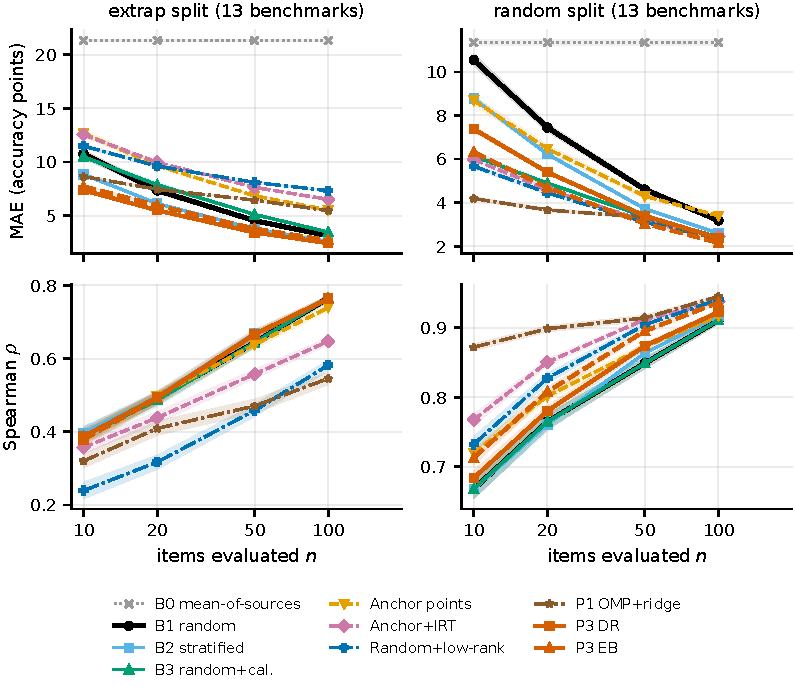
\includegraphics[width=0.8\linewidth]{../figures/generated/fig_macro_curves.pdf}
\caption{Macro-average over the 13 benchmarks of MAE (top) and Spearman correlation (bottom) against the number of items $n$ ($n\le100$), extrapolation split (left) and random split (right), 95\% bands over repetitions.}
\label{fig:macro}
\end{figure}

\subsection{Extrapolation: model-based predictors lose to random sampling}
When the targets are the strongest models, the picture changes (Table~\ref{tab:macro}, Appendix Figure~\ref{fig:paired} left). At $n=50$ the macro MAE of Anchor points, Anchor+IRT, random+low-rank and OMP+ridge is $6.85$, $7.64$, $8.10$ and $6.45$ points, against $4.54$ for B1; the paired differences are $+2.31$, $+3.10$, $+3.56$ and $+1.91$ points, and they are worse than B1 on 7, 11, 10 and 9 of 13 benchmarks. They stay worse as $n$ grows (random+low-rank: $+4.95$ at $n{=}200$). Their Spearman correlation drops to $0.46$--$0.64$ against $0.64$ for B1 and is below B1 by $0.09$--$0.19$ at $n{=}50$ for the three model-based methods. The scatter plots (Appendix Figure~\ref{fig:scatter}) show the cause: the strongest targets are predicted too low, a mean signed error of Anchor+IRT of $-12.2$ points for the targets in the top quartile of true accuracy within each benchmark and $-6.3$ for the others (pooled over benchmarks and repetitions; \texttt{figures/generated/fig\_scatter\_extrap\_bias.csv}), and, in terciles of the targets of each benchmark, $-5.0$, $-7.2$ and $-10.6$ (\texttt{q4\_by\_true\_tercile.csv}). Calibration (B3) also becomes worse than B1 ($+0.58$ points at $n{=}50$, interval $[0.39,0.77]$).

What survives is the design-based residual correction and, for the plain mean, stratification. Table~\ref{tab:ablation} separates the ingredients (13 benchmarks, TB intervals, $n{=}50$ unless stated). Without the correction the low-rank model is $+3.56$ points above B1 ($[3.37,3.74]$) with random items and $+3.54$ ($[3.35,3.73]$) with stratified items, so stratification does not protect it. Adding the correction brings it to $-0.99$ ($[-1.14,-0.83]$) with random items and $-1.10$ ($[-1.27,-0.94]$) with stratified items (P3 DR); the correction changes the MAE by $-4.55$ and $-4.65$ points. Stratification gives $-0.77$ ($[-0.95,-0.61]$) with the plain mean (B2), but given the correction only $-0.12$ ($[-0.20,-0.03]$) at $n{=}50$, and nothing distinguishable from zero at $n{=}20$ ($-0.01$, $[-0.18,0.15]$) and $n{=}100$ ($-0.04$, $[-0.10,0.02]$; these contrasts use repetition-only intervals). P3 EB, which shrinks the correction, is $0.36$ ($[0.32,0.40]$) worse than P3 DR under extrapolation and $0.36$ better on the random split. The robustness to extrapolation therefore comes from the correction, for which a random subset suffices, and stratification adds a gain mostly when the estimator is the plain mean; our earlier reading, that stratification carries P3's gain, is not supported. Against B2, P3 DR is better by $1.48$ points at $n{=}10$ (13 of 13 benchmarks; repetition-only intervals, since $n{=}10$ was not in the two-level bootstrap) but by only $0.33$ at $n{=}50$ (TB: below zero on 8 of 13 benchmarks, above on none) and $0.14$ at $n{=}100$ (6 of 13); P3 EB is not better than B2 under extrapolation at $n\ge50$ ($+0.03$, $[-0.07,0.11]$ at $n{=}50$ with 5 of 13 benchmarks worse; $+0.12$, $[0.06,0.18]$ at $n{=}100$). Against B1, none of B2, P3 DR, P3 EB or random+low-rank+correction has a TB interval above zero in any of the 78 cells (13 benchmarks $\times$ 2 splits $\times$ 3 budgets), so ``never significantly worse than B1'' holds; ``better on every benchmark'' does not: P3 DR has a TB interval below zero on 13 of 13 benchmarks at $n{=}50$ (both splits) and at $n{=}100$ on the random split, but on $10$--$12$ of 13 in the other cells (extrapolation: $11$, $13$ and $10$ at $n{=}20,50,100$; random: $12$, $13$, $13$); P3 EB on only $6$ of 13 at $n{=}50$ under extrapolation. The Spearman correlations of B2, P3 DR and P3 EB are $0.02$--$0.03$ above those of B1 at $n{=}50$ with TB intervals that reach zero for P3 DR and P3 EB (Appendix Table~\ref{tab:metrics}). So, on the extrapolation split, the source data buy a modest gain in error and nothing detectable in ranking, which answers Q1 and Q3; RMSE and Kendall give the same conclusions (Appendix Table~\ref{tab:metrics}).

\begin{table}[t]
\caption{Ablation of P3 on the 13 Tier-1 benchmarks: MAE difference to the random subset mean B1 (points; negative is better), with 95\% two-level (repetitions, then target models) bootstrap intervals, and contrasts between estimators (repetition-only intervals, same sign convention: first minus second). Generated by \texttt{paper/make\_tables.py} from \texttt{results/tables/review/}.}
\label{tab:ablation}
\centering
\resizebox{\linewidth}{!}{{\scriptsize\setlength{\tabcolsep}{2pt}
\begin{tabular}{lrrrrrr}
\toprule
 & \multicolumn{3}{c}{random split} & \multicolumn{3}{c}{extrapolation} \\
\cmidrule(lr){2-4}\cmidrule(lr){5-7}
Estimator (difference in MAE to B1, points) & $n{=}20$ & $n{=}50$ & $n{=}100$ & $n{=}20$ & $n{=}50$ & $n{=}100$ \\
\midrule
B2 stratified (plain mean) & -1.22\,{\tiny[-1.45,-0.99]} & -0.88\,{\tiny[-1.04,-0.73]} & -0.59\,{\tiny[-0.69,-0.48]} & -1.23\,{\tiny[-1.53,-0.92]} & -0.77\,{\tiny[-0.95,-0.61]} & -0.54\,{\tiny[-0.68,-0.42]} \\
Random + low-rank (no correction) & -3.00\,{\tiny[-3.19,-2.79]} & -1.50\,{\tiny[-1.64,-1.35]} & -0.82\,{\tiny[-0.92,-0.71]} & +2.26\,{\tiny[+1.94,+2.57]} & +3.56\,{\tiny[+3.37,+3.74]} & +4.20\,{\tiny[+4.06,+4.33]} \\
Random + low-rank + correction & -2.01\,{\tiny[-2.18,-1.82]} & -1.13\,{\tiny[-1.26,-0.99]} & -0.78\,{\tiny[-0.88,-0.70]} & -1.84\,{\tiny[-2.15,-1.56]} & -0.99\,{\tiny[-1.14,-0.83]} & -0.64\,{\tiny[-0.76,-0.52]} \\
Stratified + low-rank (no correction) & -3.07\,{\tiny[-3.29,-2.83]} & -1.54\,{\tiny[-1.70,-1.38]} & -0.82\,{\tiny[-0.93,-0.72]} & +2.31\,{\tiny[+2.01,+2.61]} & +3.54\,{\tiny[+3.35,+3.73]} & +4.18\,{\tiny[+4.03,+4.31]} \\
P3 DR (stratified + low-rank + correction) & -2.05\,{\tiny[-2.28,-1.81]} & -1.20\,{\tiny[-1.36,-1.05]} & -0.81\,{\tiny[-0.92,-0.71]} & -1.85\,{\tiny[-2.17,-1.55]} & -1.10\,{\tiny[-1.27,-0.94]} & -0.68\,{\tiny[-0.81,-0.55]} \\
P3 EB (shrunk correction) & -2.75\,{\tiny[-2.97,-2.52]} & -1.56\,{\tiny[-1.72,-1.40]} & -1.03\,{\tiny[-1.13,-0.93]} & -1.39\,{\tiny[-1.72,-1.08]} & -0.74\,{\tiny[-0.92,-0.58]} & -0.42\,{\tiny[-0.55,-0.28]} \\
\midrule
Contrast: DR correction, given random items & +0.99\,{\tiny[+0.93,+1.06]} & +0.37\,{\tiny[+0.32,+0.42]} & +0.03\,{\tiny[-0.01,+0.07]} & -4.10\,{\tiny[-4.24,-3.97]} & -4.55\,{\tiny[-4.64,-4.46]} & -4.84\,{\tiny[-4.91,-4.77]} \\
Contrast: DR correction, given stratified items & +1.02\,{\tiny[+0.95,+1.08]} & +0.34\,{\tiny[+0.29,+0.38]} & +0.01\,{\tiny[-0.02,+0.05]} & -4.16\,{\tiny[-4.28,-4.03]} & -4.65\,{\tiny[-4.72,-4.57]} & -4.86\,{\tiny[-4.92,-4.79]} \\
Contrast: stratification, given DR & -0.04\,{\tiny[-0.18,+0.09]} & -0.07\,{\tiny[-0.14,-0.01]} & -0.02\,{\tiny[-0.07,+0.03]} & -0.01\,{\tiny[-0.18,+0.15]} & -0.12\,{\tiny[-0.20,-0.03]} & -0.04\,{\tiny[-0.10,+0.02]} \\
Contrast: stratification, plain mean & -1.22\,{\tiny[-1.44,-1.02]} & -0.88\,{\tiny[-1.02,-0.76]} & -0.59\,{\tiny[-0.68,-0.50]} & -1.23\,{\tiny[-1.51,-0.94]} & -0.77\,{\tiny[-0.93,-0.61]} & -0.54\,{\tiny[-0.67,-0.42]} \\
Contrast: EB shrinkage vs DR & -0.70\,{\tiny[-0.73,-0.66]} & -0.36\,{\tiny[-0.38,-0.34]} & -0.22\,{\tiny[-0.24,-0.20]} & +0.46\,{\tiny[+0.40,+0.53]} & +0.36\,{\tiny[+0.32,+0.40]} & +0.26\,{\tiny[+0.23,+0.29]} \\
\bottomrule
\end{tabular}}
}
\end{table}

\subsection{Budget and items needed}
Error falls roughly as $1/\sqrt n$ for all unbiased designs (Figure~\ref{fig:curves} in the appendix). Interpolating the mean-MAE curves of each benchmark, the number of items needed to reach an MAE of $2$ points within the evaluated budgets ($n\le\min(200,N/4)$) is attained on the extrapolation split on only $4$ of 13 benchmarks for B1 (median $\approx 141$ items among them), $6$ for B2 (median $\approx 139$) and $7$ for P3 DR (median $\approx 129$); model-based methods reach it on $0$--$2$ benchmarks. On random splits, B1 reaches it on $2$ benchmarks, P3 EB on $10$ (median $\approx118$) and OMP+ridge on $6$ (median $\approx 22$ items; \texttt{results/tables/tier1/items\_needed.csv}). Hence a 2-point error needs on the order of a hundred items on many benchmarks, and in the extrapolation case it is not reached on most benchmarks within the cap $N/4$ (a limit of the grid, not a statement about larger budgets).

\subsection{Where the error comes from, and ranking}
For each target model we separate the squared bias of its prediction over repetitions from the variance over repetitions (Appendix Table~\ref{tab:q4}, $n{=}50$, mean over benchmarks and targets). Under extrapolation the IRT, low-rank and OMP methods have much lower variance ($3.8$--$7.3$ points$^2$) than B1 ($32.2$), but a squared bias of $58$--$88$ against B1's $1.2$, which is about the estimation floor for the extrapolation split (the variance of B1 divided by the $30$ draws is about $1.1$); anchor points have both a high bias ($109$) and a high variance ($23$). The design-based methods B2, P3 DR and P3 EB keep a squared bias of $0.7$--$5.9$ and cut the variance from $32.2$ to $17$--$23$. On random splits a model is a target in only about a quarter of the $30$ repetitions ($\approx7.5$ draws), so the floor for an unbiased design is about $4$ (B1: squared bias $5.1$, variance $29.9$); the squared bias is at most $14$ points$^2$ for every method but B0, and the model-based ones reduce the variance, which is why they win there.

Models closer than a few points are not ranked reliably by any method (Appendix Figure~\ref{fig:pairwise}, $n{=}50$): for pairs whose true accuracies differ by less than 1 point the fraction of correctly ordered pairs is $0.50$--$0.51$ for B1 and P3 DR in both splits, rising to $0.59$--$0.62$ for gaps of 1--2 points and to $0.71$--$0.73$ for 2--5 points on the extrapolation split; Anchor+IRT is mostly better than B1 on random splits, and Anchor+IRT and OMP+ridge are worse than B1 on the extrapolation split for gaps above 5 points. High macro rank correlations (Table~\ref{tab:macro}) therefore reflect the large spread of model accuracy and not the ability to resolve close models.

\subsection{Further analyses}
These analyses were run after the Tier-1 results and the design freeze, on subsets of the benchmarks (7 for the factorial, source-size and coverage analyses; 4 for the organisation hold-out; 5 for the rank ablation, chosen by the analysis owner for computing time) with 20 repetitions; none of them changed a Tier-1 number or the frozen P3 design. Intervals below are repetition-bootstrap intervals with fixed targets, like those above (appendix tables give the MAE values of every cell; the full tables with intervals are in \texttt{results/tables/macro/}).

\paragraph{Organisation hold-out behaves like the random split.}
We also held out all models of one organisation (the prefix of the model name; four folds, the four Open LLM Leaderboard benchmarks only, because the HELM model names carry no verifiable family label). The organisation prefix is a coarse family label, since community fine-tunes sit under other prefixes, and this split is not a capability shift. At $n{=}50$ the macro MAE on these four benchmarks is B1 $4.87$, B2 $4.20$, P3 DR $3.73$, random+low-rank $2.88$ and OMP+ridge $2.20$, almost the same as on the random split of the same benchmarks ($4.91$, $4.18$, $3.72$, $2.78$, $1.95$; Table~\ref{tab:family}) and unlike their extrapolation values ($5.21$, $4.61$, $4.18$, $10.04$, $7.16$). Across the twelve methods the Spearman correlation of their MAE between the random and the organisation hold-out split is $+0.97$ to $+1.00$ ($n{=}20,50,100$), and between the random and the extrapolation split $-0.51$ to $-0.62$: leaving out one organisation does not reproduce the reversal that leaving out the strongest models causes, so conclusions on interpolation do not transfer to capability shift.

\paragraph{Which ingredient protects against extrapolation.}
Table~\ref{tab:factorial} crosses selectors and estimators ($n{=}50$, 7 benchmarks, 20 repetitions). Under extrapolation every estimator that uses a fitted model of the sources without correction (ridge, $k$-NN, IRT, low-rank) has an MAE of $7.8$ to $12.5$ points with every selector, and calibration $5.4$ to $11.5$, against $4.65$ for random items with the subset mean. Adding the residual correction brings the same models to $3.9$--$4.1$ points with random, stratified and PPS items (random+low-rank+correction: $3.91$, paired difference to B1 $-0.74$ points, interval $[-0.88,-0.60]$; stratified+low-rank+correction $3.72$, $-0.93$, $[-1.11,-0.75]$). So the protection comes from the correction, and a random subset suffices for it; stratification, which alone gives $4.04$ with the mean ($-0.61$, $[-0.80,-0.40]$), adds a further $0.2$ points to the corrected model (a difference we did not test pairwise on this subset). The correction has a price when sources are informative: on the random split the plain low-rank model with stratified items has MAE $3.14$ and the corrected one $3.64$ (B1 $4.82$), and on all 13 Tier-1 benchmarks $3.06$ against $3.40$. Selectors that use the sources to look for informative items (OMP, c-optimal) are good only with a model estimator and are poor with the plain mean ($8.53$ and $14.91$ points on the random split), as their items are not representative of the benchmark. The Tier-1 ablations on all 13 benchmarks (Table~\ref{tab:ablation}) agree.

\paragraph{Number of source models.}
With few source models (Table~\ref{tab:ssize}; 7 benchmarks, $n{=}50$) the fitted models lose their advantage on the random split: random+low-rank has an MAE of $5.38$, $4.43$ and $3.64$ with $10$, $20$ and $40$ source models and $3.18$ with all, against $4.82$ for B1 (which does not use the sources); Anchor+IRT is at $8.08$ with $10$ sources. P3 DR is at $4.15$, $4.00$, $3.87$ and $3.63$ and P3 EB at $3.94$, $3.69$, $3.46$ and $3.18$, so the design-based methods are not worse than B1 even with $10$ sources. Under extrapolation more sources do not remove the bias of the model-only estimators ($14.24$ to $9.85$ for random+low-rank) while P3 DR stays at $4.26$--$3.75$ against $4.65$ for B1.

\paragraph{Sensitivity to the rank of the latent model.}
We varied the rank $k\in\{2,4,8,16,32\}$ of the low-rank model in the stratified designs (5 benchmarks, $n{=}50$, Table~\ref{tab:rank}; $k{=}8$ is the frozen P3 and was fixed before the results). Under extrapolation P3 DR is between $3.55$ and $3.74$ points for $k\le16$ (B1: $4.36$ on these benchmarks) and worse than B1 at $k{=}32$ ($5.09$, paired difference $+0.73$, interval $[+0.40,+1.07]$); with the shrunk correction, $k{=}32$ gives $5.68$. The plain model fails at every $k$ ($9.5$--$10.6$). On the random split all variants lie between $3.2$ and $3.7$. The robustness of the correction is therefore not a property of one particular rank, but it fails when the model is flexible enough to overfit $n{=}50$ answers.

\paragraph{Benchmark properties and interval calibration.}
The gain of P3 DR over B1 at $n{=}50$ is larger on benchmarks whose item accuracies over the source models are more spread out (Spearman $-0.91$ on the random and $-0.82$ on the extrapolation split; descriptive, 13 benchmarks), and the nominal 95\% analytic interval of a single prediction covers $0.86$--$0.94$ of the true scores, below nominal at small $n$ and on the random split (Appendix~\ref{app:further}). The intervals of this paper are bootstrap intervals over the study, not these.
